The background model uses a mixture of gaussians method, looking at all three color channels in the image.

\subsubsection{Expectation maximization}
The normal expectaion maximation algortihm is to slow to run in real time, so we use a somewhat simplified version outlined in Wood (2007)

See code in appendix \ref{sec:BGMod_code}. %referens till kod, ger klickbar länk.

\begin{figure}[htb]
	\centering
	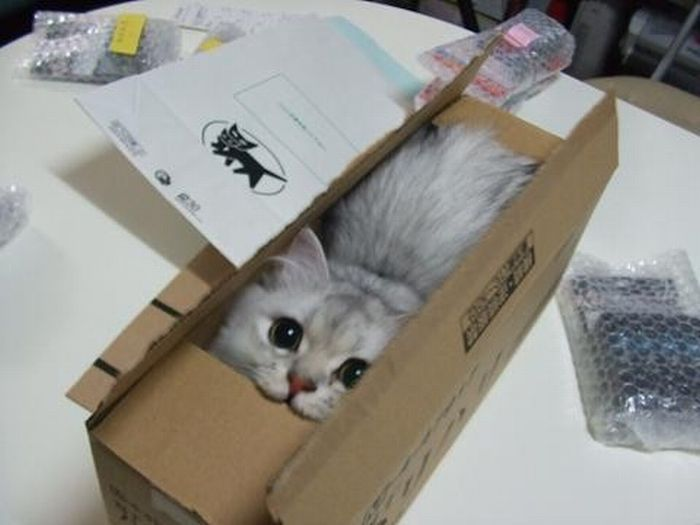
\includegraphics[width=\linewidth]{images/acatisfinetoo}
	\caption{\textit{Background modeling figure.}}
	\label{fig:BGModeling_fig} %Skapar referens till figuren
\end{figure}

\subsubsection{Moar info}
Moar info, Moar info, Moar info, Moar info, Moar info, Moar info, Moar info, Moar info, Moar info, Moar info, Moar info, Moar info, Moar info, Moar info, Moar info, Moar info, Moar info, Moar info, Moar info, 
This can be seen in figure \ref{fig:BGModeling_fig}. %Referens till figur, Ger klickbar länk i pdfen.
